\documentclass[a4j,11pt,twoside]{jbook}
\usepackage{ascmac}
\usepackage[dvipdfmx]{graphicx}
\usepackage{matx}
\usepackage{manyfloat}
\usepackage{caption}
\captionsetup{labelformat=empty,labelsep=none}

\begin{document}

%--- title page ---%
\title{倒立振子の安定化制御}
\author{前田 拓}
\date{2017年7月12日}
\maketitle

%--- index ---%
\pagenumbering{roman}
\tableofcontents
\listoffigures
\listoftables
\pagenumbering{arabic}

%--- main ---%
\chapter{はじめに}
\section{目的}
本実験の目的は、倒立振子系を状態空間表現を用いて安定化制御し、線形不変システムを設計することである。
具体的に、次のことを目的とする。
\begin{itemize}
    \item 倒立振子が安定化制御を行っている状態において、外乱による影響で振子が傾いたとき、倒立状態に戻すことができる (不安定平衡点の安定化)。
    \item 倒立振子系に一定周期のパルス入力を与え、台車を目的の変位へ移動させる。
    \item 倒立振子が入力なしで静止している状態から、台車を動かすことにより振子を振り上げ、倒立状態にする (振り上げ制御)。
\end{itemize}
\section{実験装置}
\begin{figure}[htbp]
    \begin{center}
        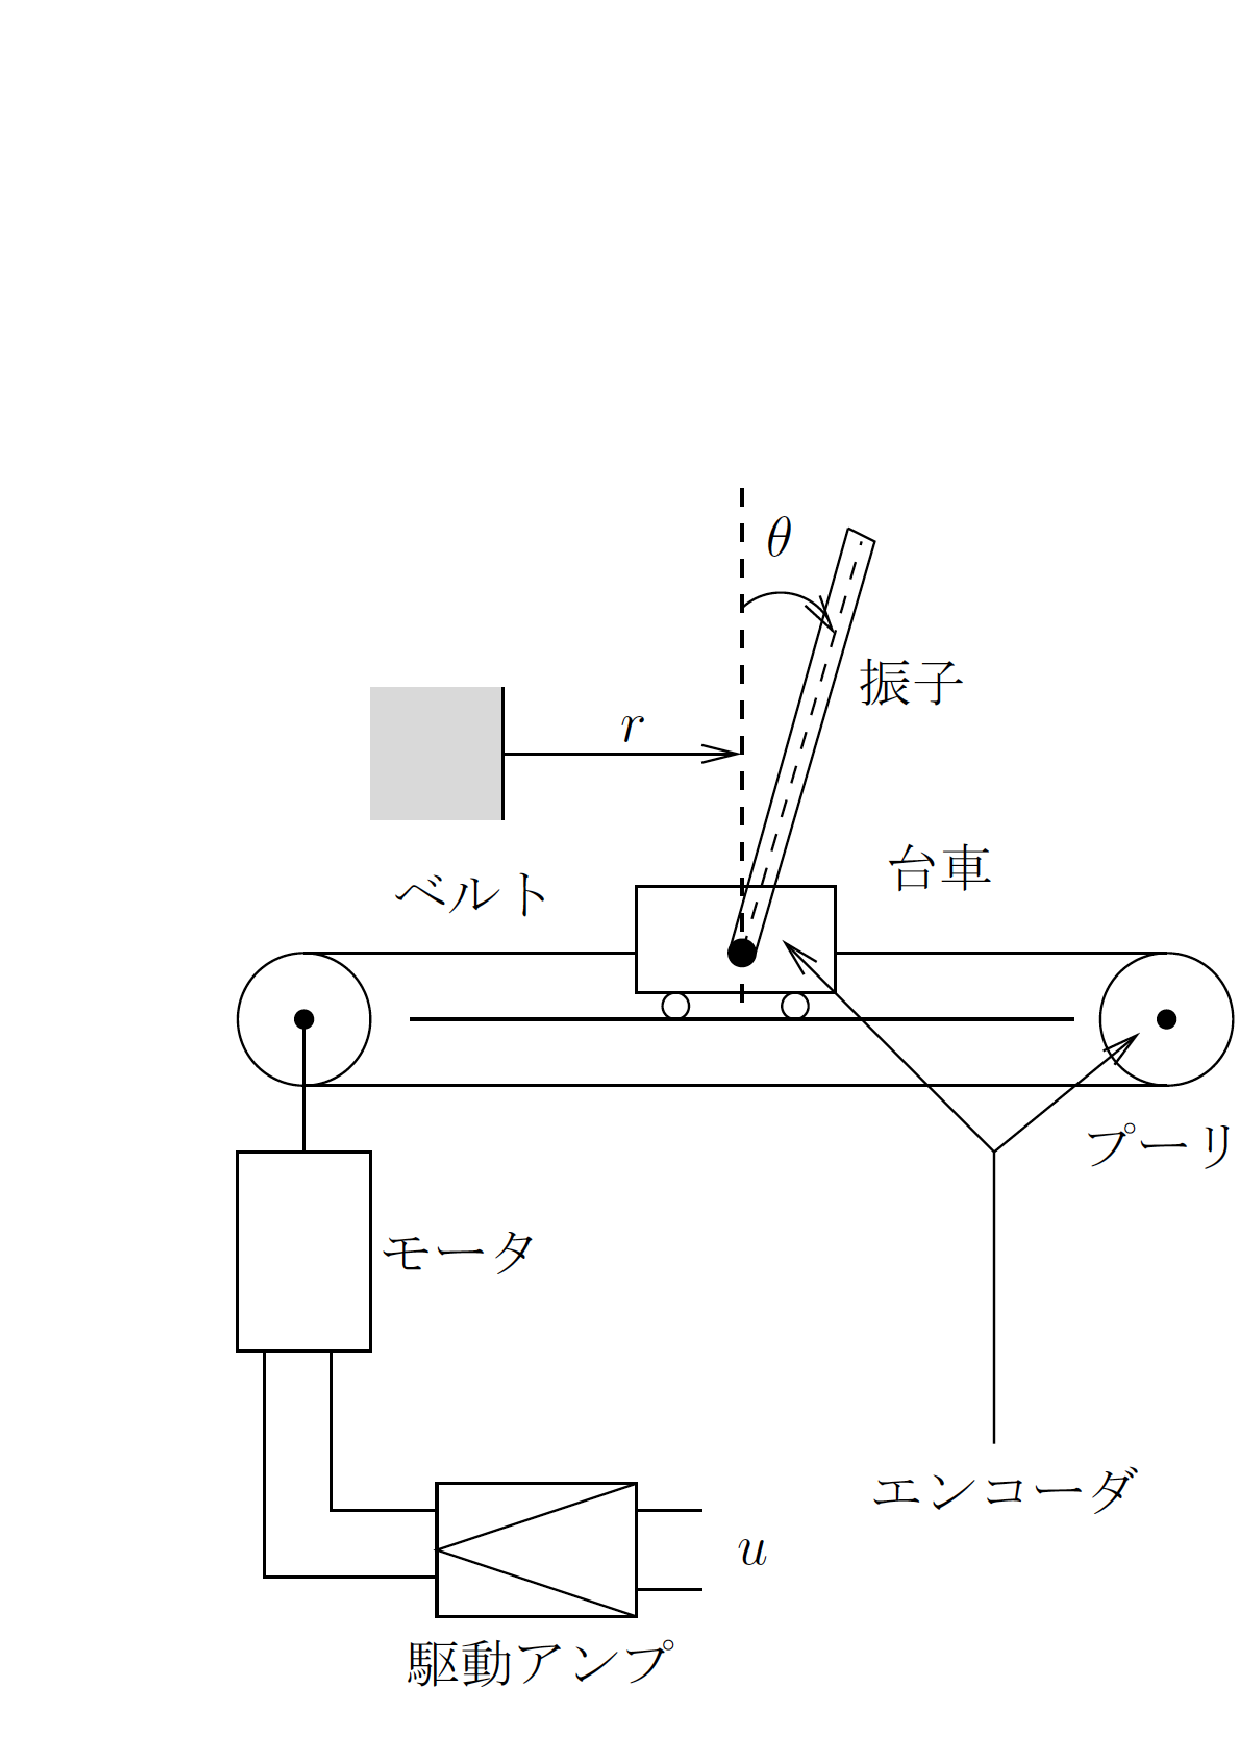
\includegraphics[width=0.6\linewidth]{model.png}
        \caption{図\ref{pendulum}: 倒立振子系}
        \label{pendulum}
    \end{center}
\end{figure}

図\ref{pendulum}は本実験で使用する倒立振子系である。
系は、モータ、ベルト、プーリ系から成り、台車はモータからの入力によりベルト上を水平方向に動くことができる。
台車の初期状態からの変位を$r$とする。
また、鉛直方向上向きから時計回りを正の方向として、台車に取り付けられた振子が回転した角度を$\theta$とする。
ポテンショメータにより、$r$と$\theta$を測定し、入力$u$を与える。

\chapter{モデリング}
\section{数式モデル}
制御器の設計のため、倒立振子系の状態方程式、観測方程式から数式モデルを導出する。
\begin{figure}[htbp]
    \begin{center}
        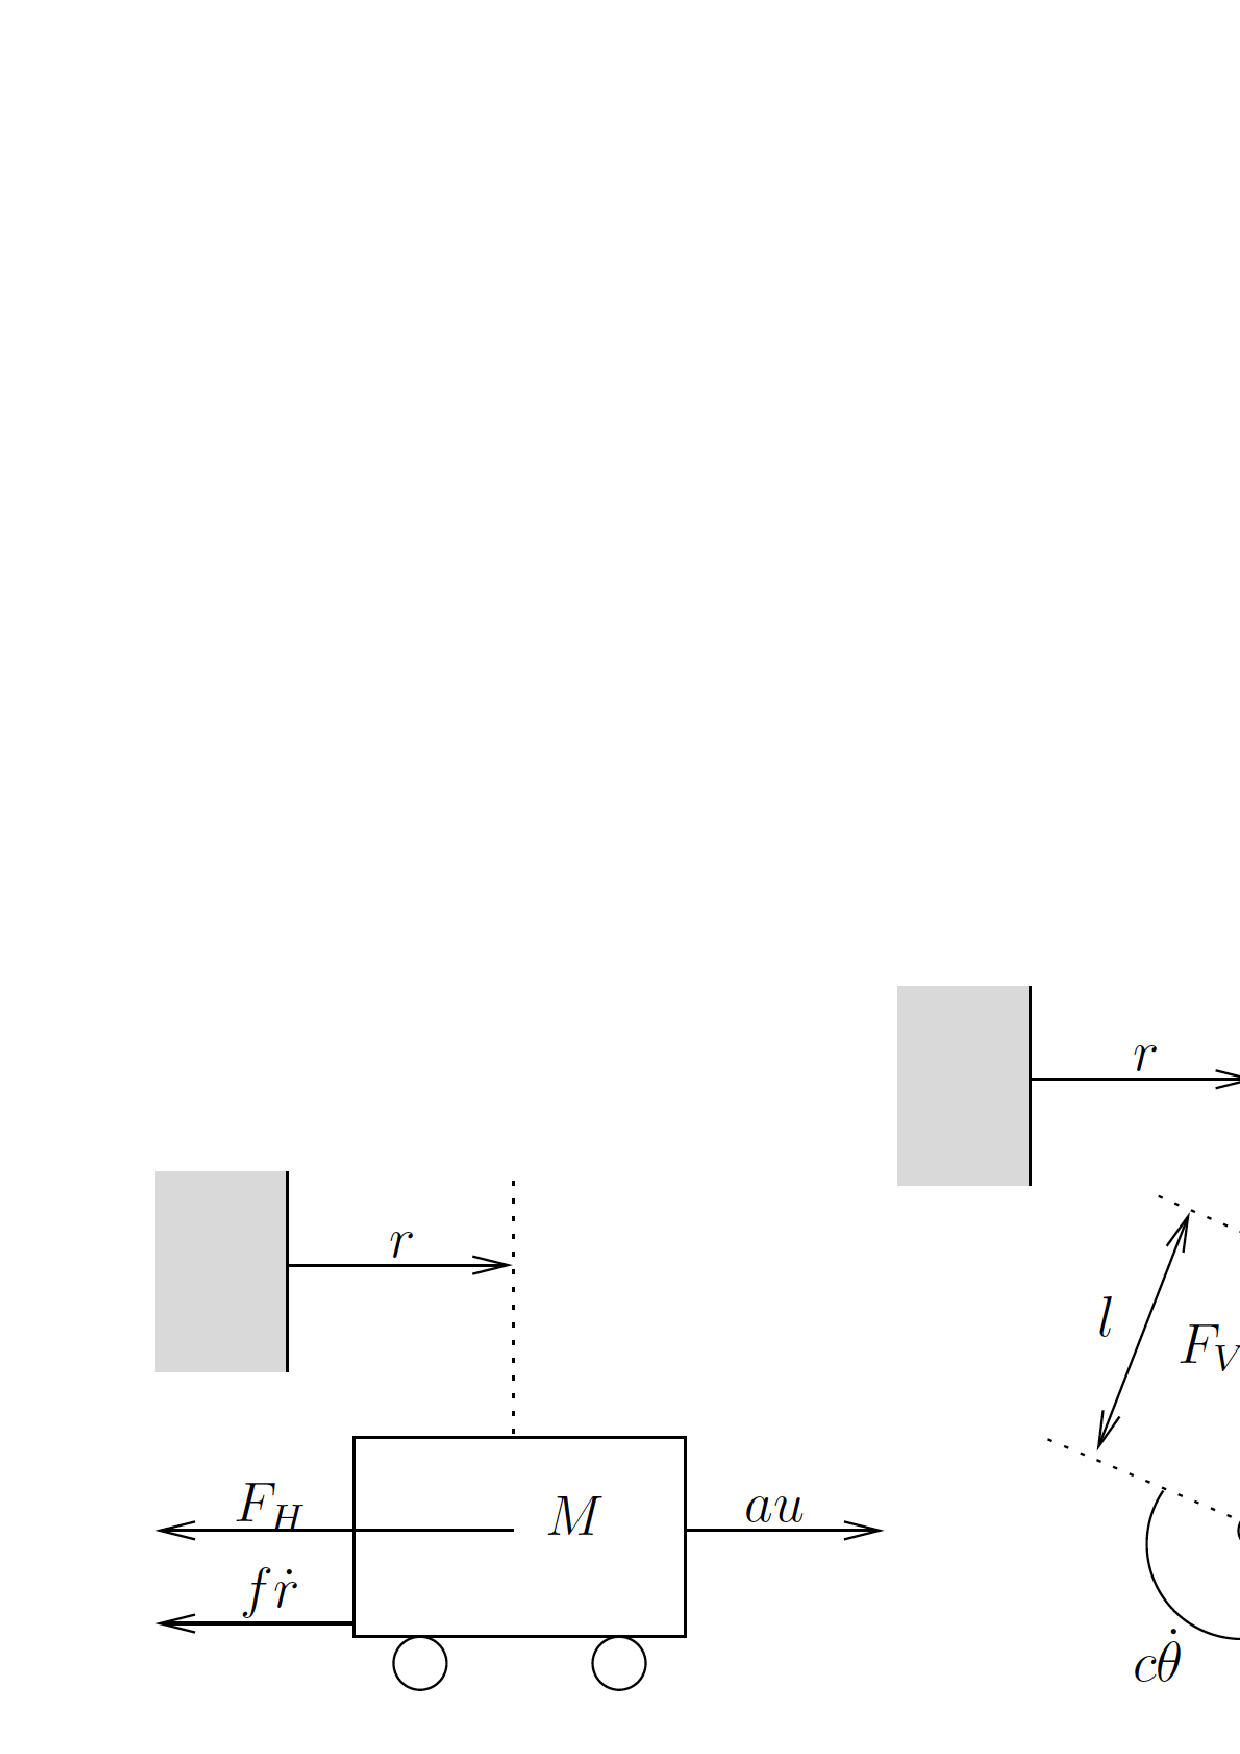
\includegraphics[width=0.6\linewidth]{modeling.png}
        \caption{図\ref{modeling}: モデリングのための力の分解}
        \label{modeling}
    \end{center}
\end{figure}

図\ref{modeling}から導出した倒立振子系の運動方程式を
式(\ref{modeling:cart1})から式(\ref{modeling:pend2})に示す。

\begin{equation}
    M \ddot r = au - F_{H} - f \dot r
    \label{modeling:cart1}
\end{equation}
\begin{equation}
    J \ddot \theta = lF_{V}\sin \theta - lF_{H}\cos \theta - c \dot \theta
    \label{modeling:pend1}
\end{equation}
\begin{equation}
    m\frac{d^2}{dt^2}(r + l\sin \theta) = F_{H}
    \label{modeling:cart2}
\end{equation}
\begin{equation}
    m\frac{d^2}{dt^2}(l\cos \theta) = F_{V} - mg
    \label{modeling:pend2}
\end{equation}

ただし、$M$,$f$は台車の質量と摩擦係数、$m$,$l$,$c$,$J$は振子の質量、振子の重心から回転軸までの距離、
回転軸摩擦係数、重心周りに働く慣性モーメントである。また、$F_{H}$,$F_{V}$は振子が台車から受ける
水平効力と垂直抗力である。$F$はモータによる台車への駆動力であり、定数$a$、駆動アンプへの入力電圧$u$を用いて
式(\ref{F})で表される。

\begin{equation}
    F = au
    \label{F}
\end{equation}

ここで、系の状態$x$を4つの状態変数からなる縦ベクトルとする。すなわち、
$$
    x = \left [
    \begin{array}{c}
        r \\
        \theta \\
        \dot r \\
        \dot \theta
    \end{array}
    \right ]
$$
と定義する。
次に、式(\ref{modeling:cart1})から式(\ref{modeling:pend2})から倒立振子系の非線形方程式を求める。
式(\ref{modeling:cart1}),式(\ref{modeling:pend1})から$F_{H}$を消去すると、
$$
    M \ddot r = au - m \ddot r + ml \sin \theta - f \dot r
$$
となり、式(\ref{ddot_r})が得られる。
\begin{equation}
    \ddot r = \frac{au + ml\sin \theta - f \dot r}{M + m}
    \label{ddot_r}
\end{equation}
また、式(\ref{modeling:pend1}),式(\ref{modeling:cart2}),式(\ref{modeling:pend2})から
$F_{H}$,$F_{V}$を消去すると、
$$
    J \ddot \theta = l\left(
        m\frac{d^2}{dt^2}\left(
            l\cos \theta + mg
            \right)
        \right)\sin \theta
        -
        l\left(
            m\frac{d^2}{dt^2}\left(
                r + l\sin \theta
            \right)
        \right)\cos \theta
$$
となり、式(\ref{del_Fh_Fv})が得られる。
\begin{equation}
    ml\cos \theta \ddot r + (J + ml^2) \ddot \theta = mgl\sin \theta -c \dot \theta
    \label{del_Fh_Fv}
\end{equation}

\chapter{制御系設計}

\chapter{シミュレーション}

\chapter{実験}

\chapter{おわりに}

\end{document}
